\section{The Power of Parametric Memory for Complex Reasoning}

\label{sec:hard_reasoning}

At the high level, our study so far paves the way towards better understanding and improving transformer's reasoning with \textit{parametric} representation of knowledge and rules. But why is parametric memory practically important? Can we not simply enhance LLMs with non-parametric memory, e.g., by using their long-context modes and/or doing explicit retrieval, to solve the tasks at hand?

We believe parametric memory has its unique capability to perform \textit{deep compression and integration of information} for complex reasoning.
To showcase the potential of parametric memory for complex reasoning, we create a difficult reasoning task with a \textit{large search space}, and show that 1) it is far out of reach even for current SoTA models (e.g., GPT-4-Turbo~\citep{openai_devday_2023} and Gemini-Pro-1.5~\citep{google2024gemini}) based on non-parametric memory; 2) a fully grokked transformer can solve the task with near-perfect accuracy.

Our task is a variation of the comparison task above where we use a simple way to massively expand the search space, based on an additional set of rules that are already contained within the task itself, namely, the \textit{(anti-)symmetry} and \textit{transitivity} of comparison:
\begin{equation}
\label{eq:comparison_2}
\begin{aligned}
    \forall e_1,e_2 \in \mathcal{E}, \forall a\in \mathcal{A}, (a, e_1, e_2, a_</a_=/a_>)  \implies& (a, e_2, e_1, a_>/a_=/a_<), \\
    \forall e_1,e_2,e_3 \in \mathcal{E}, \forall a\in \mathcal{A}, \forall y\in \{a_<, a_=, a_>\}, (a, e_1, e_2, y)  & \land (a, e_2, e_3, y) \implies (a, e_1, e_3, y).\\
\end{aligned}
\end{equation}

In the original setting (\S\ref{sec:comparison}) of the task, for the OOD test set, one can simply retrieve the two OOD facts and compare the attribute values, which requires no further search. We change the task setting via the following. For each attribute, 1) we do \textit{not} add the OOD atomic facts into training, and 2) we add a random portion of the comparisons between ID entities and OOD entities into training. We test the models on queries consisting of \textit{derivable} (from all training facts) comparisons between OOD entities where any possible proof would involve rules from \textit{both} Eqs.(\ref{eq:comparison}) and Eqs.(\ref{eq:comparison_2}). Consequently, answering a test query would require the model to successfully \textit{locate two ID bridge entities} which can connect the two query entities into a proof (Figure~\ref{fig:cmlx}). We select a balanced (by $a_<,a_=,a_>$) subset from these queries for evaluation. More details are included in Appendix~\ref{app:hard_reasoning}.

\begin{figure}[h]
\centering
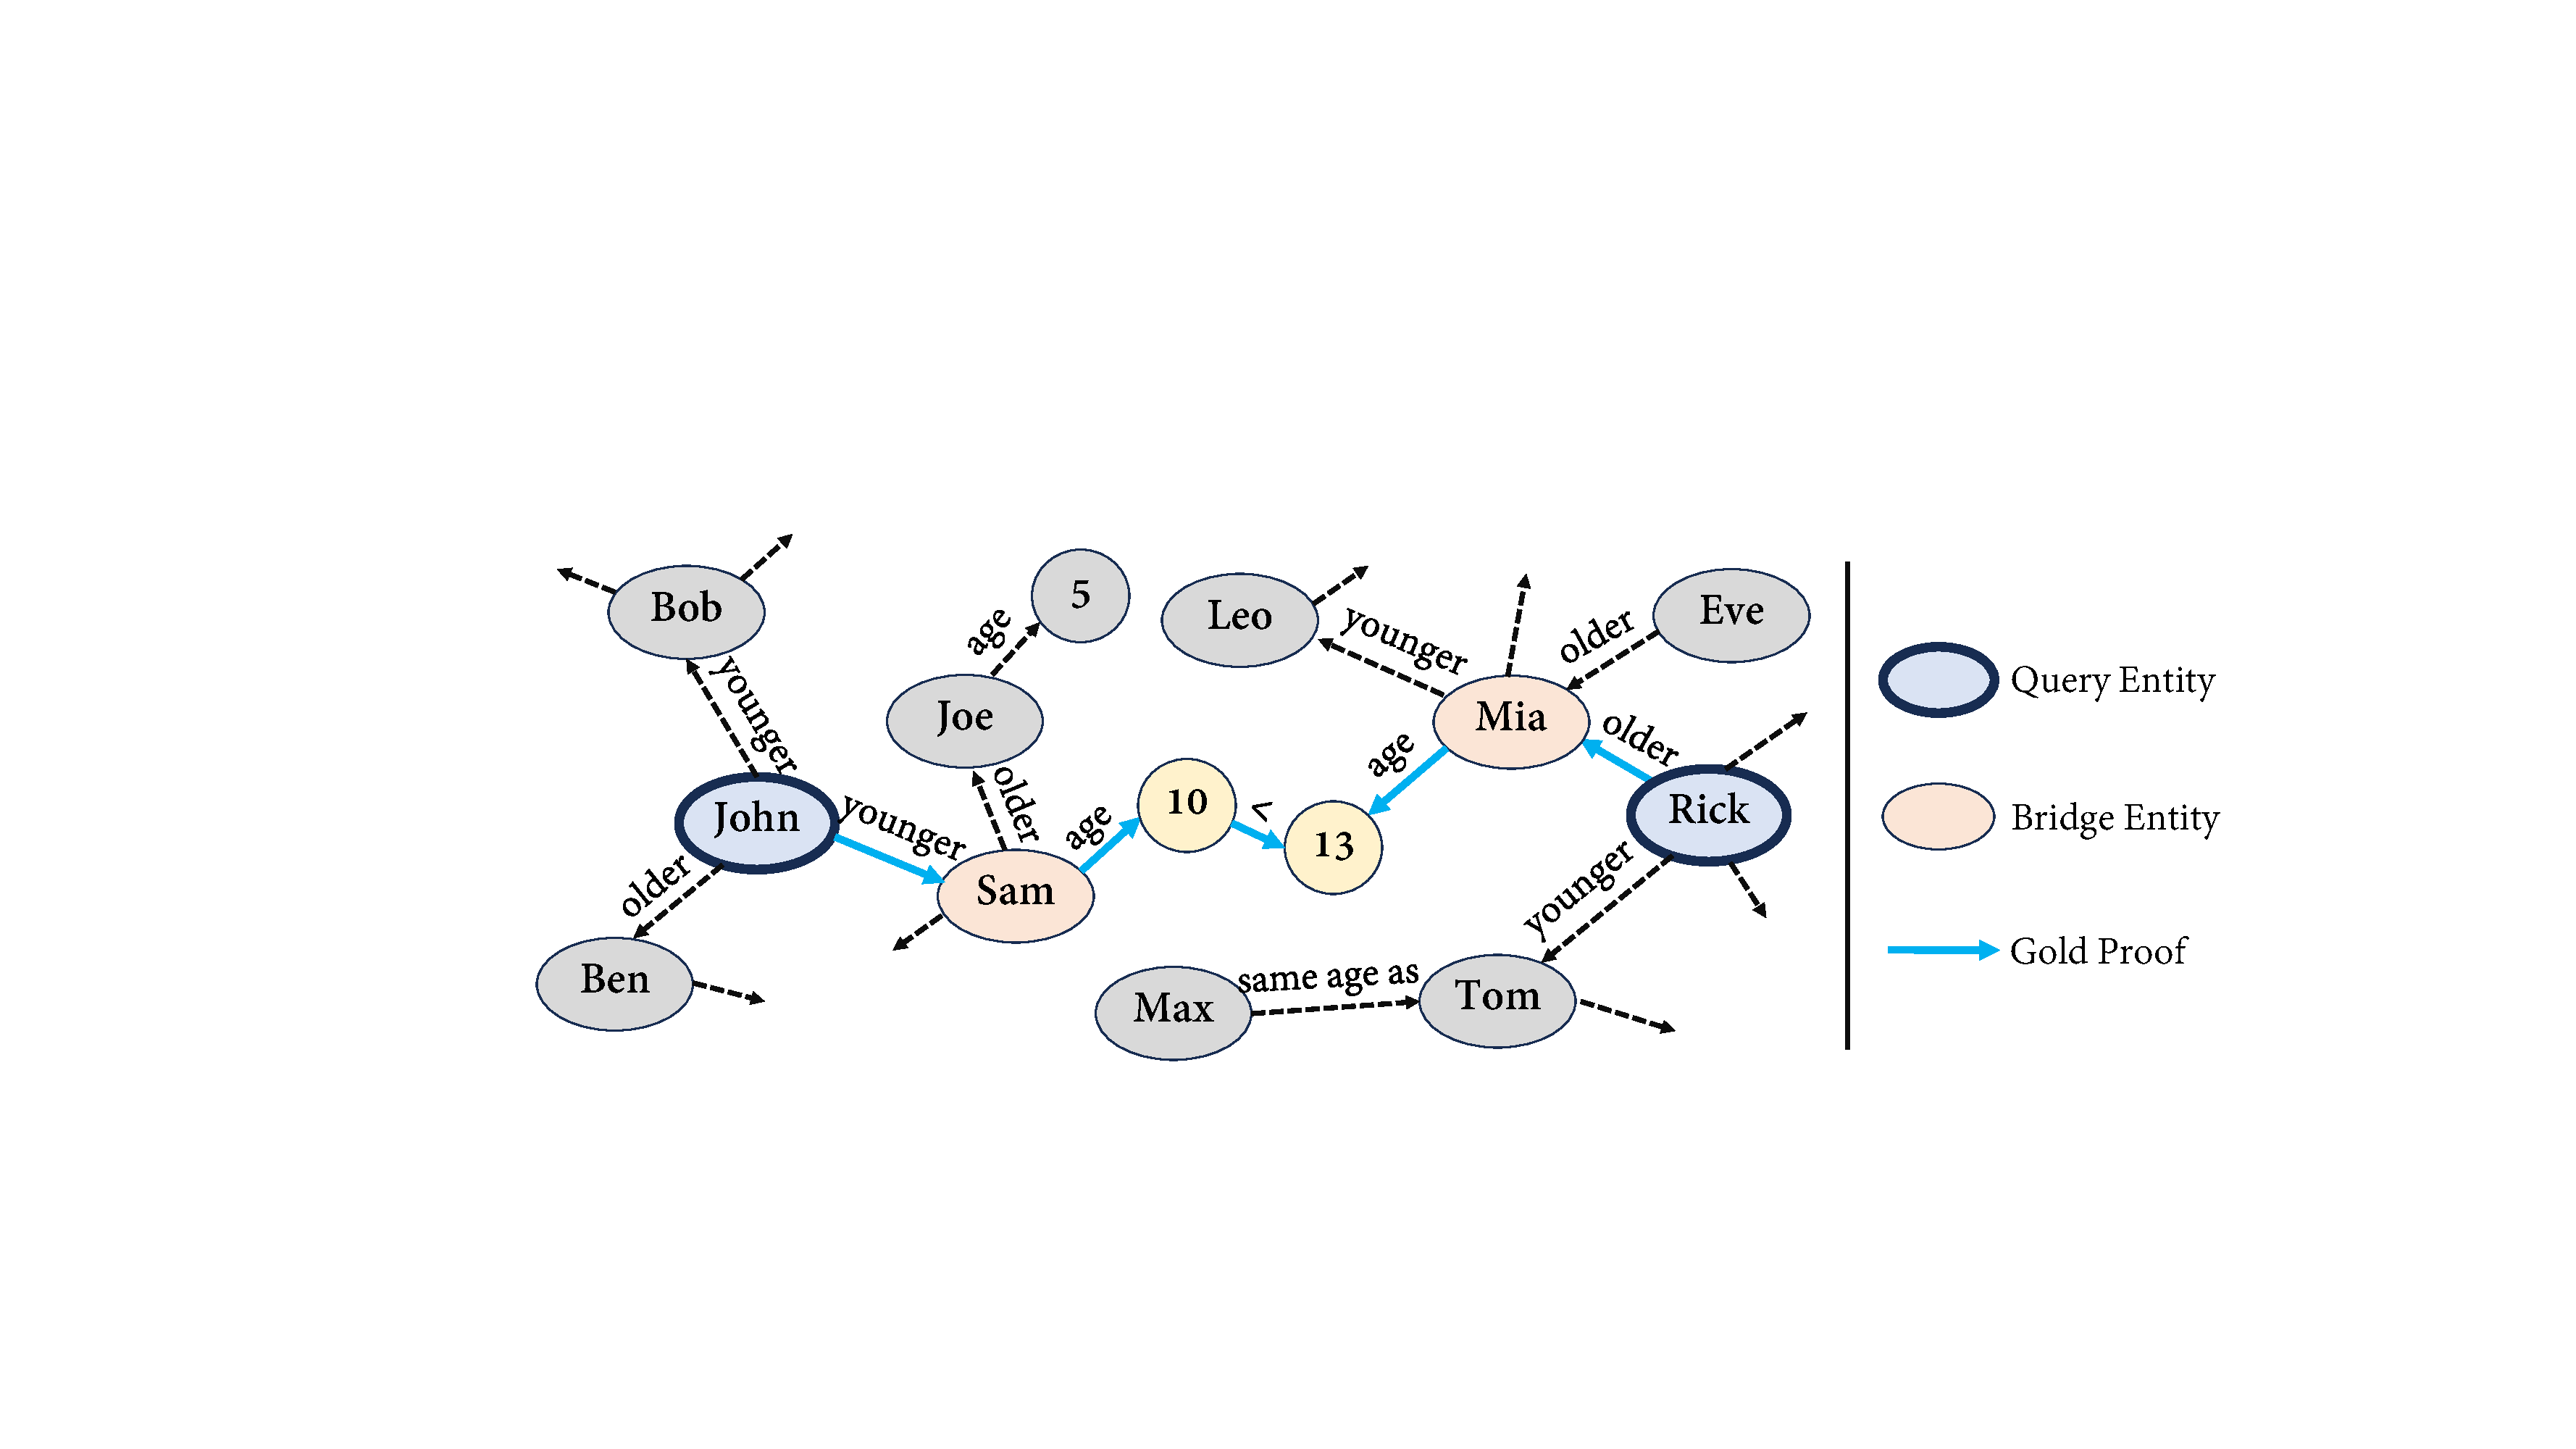
\includegraphics[width=0.77\textwidth]{fig/cmlx.pdf}
\caption{Illustration of the complex reasoning task, which involves comparing the attributes of two query entities based on a set of facts encompassing a large search space.}
\label{fig:cmlx}
\end{figure}


The difficulty of such a task is two-fold. First, the search space is large. For example, on average, each query entity connects with more than \num{50} facts, and each bridge entity in the ground truth proof connects with more than \num{900} facts. Second, there are \textit{no surface form clues} to exploit and bias the search towards the ground truth proof, unlike most conventional QA benchmarks where the proof steps are transparent from the query.

To test LLMs based on non-parametric memory, we translate the facts into natural language by simple templates (Appendix~\ref{app:hard_reasoning}). Facts/queries for each attribute are grouped/tested separately.\footnote{This could also be thought of as performing a retrieval step into the memory based on the attribute.} We test both the vanilla setup where all facts (\num{28.2}K on average) are loaded into the LLM context, and the retrieval-augmented setup (\num{5.4}K facts retrieved on average) where the two-hop neighborhoods of the two query entities are retrieved, which includes enough facts to deduce the answer. We also try both standard prompting where the model answers directly, and chain-of-thought (CoT) prompting where the model is prompted to verbalize the reasoning. We test GPT-4-Turbo and Gemini-Pro-1.5, where for GPT-4-Turbo we only test the retrieval-augmented setup due to context length limit.

% \vspace{-10pt}
\begin{table}[h]
\caption{Results on the complex reasoning task. Direct/CoT: predict the answer directly/verbalize the reasoning steps. ``+R'': retrieval augmentation.}
\centering
\resizebox{1.0\textwidth}{!}{
\begin{tabular}{lccccccc}
\toprule
     &\multicolumn{2}{c}{\textbf{GPT-4-Turbo}}&\multicolumn{4}{c}{\textbf{Gemini-Pro-1.5}}& \multirow{2}{*}{\textbf{Grokked Transformer} }  \\
     \cmidrule(l{0.5em}r{0.5em}){2-3}\cmidrule(l{0.5em}r{0.5em}){4-7} %\cmidrule(l{0.5em}r{0.5em}){8-9}
     & Direct+R & CoT+R & Direct & CoT & Direct+R & CoT+R &  \\
     \midrule
     \textbf{Accuracy (\%)}&33.3 & 31.3 & 28.7 & 11.3&37.3 & 12.0&\textbf{99.3}\\
     \bottomrule
\end{tabular}
}
\label{tbl:hard_reasoning}
\end{table}
% \vspace{-10pt}

\noindent\textbf{Results}. As shown in Table~\ref{tbl:hard_reasoning}, all models based on non-parametric memory fail badly, where the only setting that surpasses random guess (\num{33.3}\%) is the retrieval-augmented setting with Gemini-Pro-1.5 and direct answer prediction. Intriguingly, LLMs perform worse (especially Gemini) when prompted to reason verbally. Through closer examinations, we find that with CoT, \num{70.7}\% of Gemini's responses conclude that the answer cannot be decided (which we treat as wrong since the answer can be decided) after a series of search steps.\footnote{The ratio drops a bit to \num{58.7}\% when augmenting with retrieval.} More shockingly, \textit{most of the CoT rationales that achieve the correct final answer are actually wrong due to either hallucinating underivable facts or logical errors}. This illustrates the current models' inability to reason deeply with non-parametric memory. On the other hand, a grokked transformer, which is trained extensively on the given facts to compress and integrate the information to the extreme, could achieve near-perfect accuracy. By examining the model, we find that it acquires the same generalizing circuit as in Figure~\ref{fig:circuit_comparison}(a), and remarkably, even though not explicitly encouraged/trained to do this, the model successfully infers most of the OOD entities' attribute values by integrating the observed training facts (Appendix~\ref{app:hard_reasoning}).